\documentclass[12pt]{article}
\usepackage[english]{babel}
\usepackage{graphicx, amsmath, amsfonts, amsthm, mathtools, listings, color, caption, rotating, subfigure, fullpage, textcomp, enumerate, float, listings, hyperref, MnSymbol, wasysym}

\begin{document}
\begin{center}
Cats and Dogs Final Report\\
June 9, 2014, STA298\\
Christopher Aden, Chuan Qi, Nick Ulle\\
\end{center}

\section{Introduction}
The Cats and Dogs problem intially comes from Kaggle.com's Dogs vs. Cats competition. The purpose of the comeptition was to gauge how far along image recognition has come in detecting dogs versus cats (a task proposed as an alternative to reCAPTCHA to verify that a user is a human and not a computer). Using support vector machines, (Golle, 2008) was able to achieve 82.7\% classification rate, training on color and texture features from an image. Our training set involves 20,000 images: pictures of dogs and cats with file names indicating whether they were a dog or cat. Our test set consists of 5,000 images with no tags. The objective is to determine whether an image in the test set is a cat or a dog, with a high degree of accuracy, based on a model created using the training data.

The purpose of this project is to demonstrate that deep learning is a more effective method for classifying images than the previous standard established in Golle's paper. 

\section{Approaches--The Successful and The Failed}
We tried four fundamentally different approaches to classifying the images. While we ultimately decided to use the OverFeat software for classification, we originally considered implementing our own algorithm as well. The intention was that we could find something with better interpretability, albeit with some loss of accuracy.

\subsection{K-means}
One approach we found for this, from (Coates \& Ng, 2012), was to use spherical k-means clustering for feature extraction. In particular, each image in the training set is divided into 16 by 16 patches of pixels, and spherical k-means clustering is applied to produce a dictionary of features. To classify a test image, first each patch of the image is mapped to an entry in the feature dictionary. Many different mappings are possible; typically there is some trade-off between efficiency and accuracy. The number of occurrences of each feature can then be counted---although this is not the only approach---and provided to an appropriately-trained linear classifier.

This k-means-based approach to the problem had the potential to be easily interpretable: our hope was that many patches in the feature dictionary would have a clear correspondence to either cats or dogs. Moreover, the original paper was flexible to the needs of the reader. A wide array of possibilities for tuning and adjusting were presented, which would have given us many avenues for improving accuracy.

Spherical k-means clustering is sufficiently exotic that we could find no pre-existing libraries implementing it, so we wrote our own implementation. A major concern was how well the algorithm would scale to our very large training set, and we made preliminary investigations into moving our
Python code to Cython.

Due to the astounding success of OverFeat on the data set, this was as far as we got with implementing the k-means clustering strategy.

\subsection{Pixel-Based Classifiers}
A very simple approach to classification is to work on the pixel level. Using the \verb+Image+ library in Python, we can turn each image into three matrices, each one with number of rows equal to the number of pixels wide the image is, and columns equal to the image's pixel height. The three matrices correspond to the intensity of red, blue, and green in the $(i,j)$ pixel. We then flatten each image into a width x height x 3 array of RGB pixel intensities. 

Doing this for all images in the training data, we then stack them into a matrix, scaling to make them all have the same width and height. The resolution chosen was 500 x 350, which was somewhat arbitrary. It was the mean resolution of ten arbitrarily-chosen images. Without the images being the same resolution, we would not have been able to put them all in a matrix.

This is now a very high dimensional classification, where we are attempting to predict a binary response (dog or cat) using the pixel intensities from the $500 \cdot 350 \cdot 3 = 525,000$ pixel dimensions. To reduce the ill-fitting nature of this classification, we apply principal components analysis to the pixel intensities. The hope is that the first few principal components of the dogs looks different from the first few principal components of the cats, and that we can use some discriminant to split them apart. The following plot shows the first two principal axes using this strategy.

\begin{figure}[H] \center
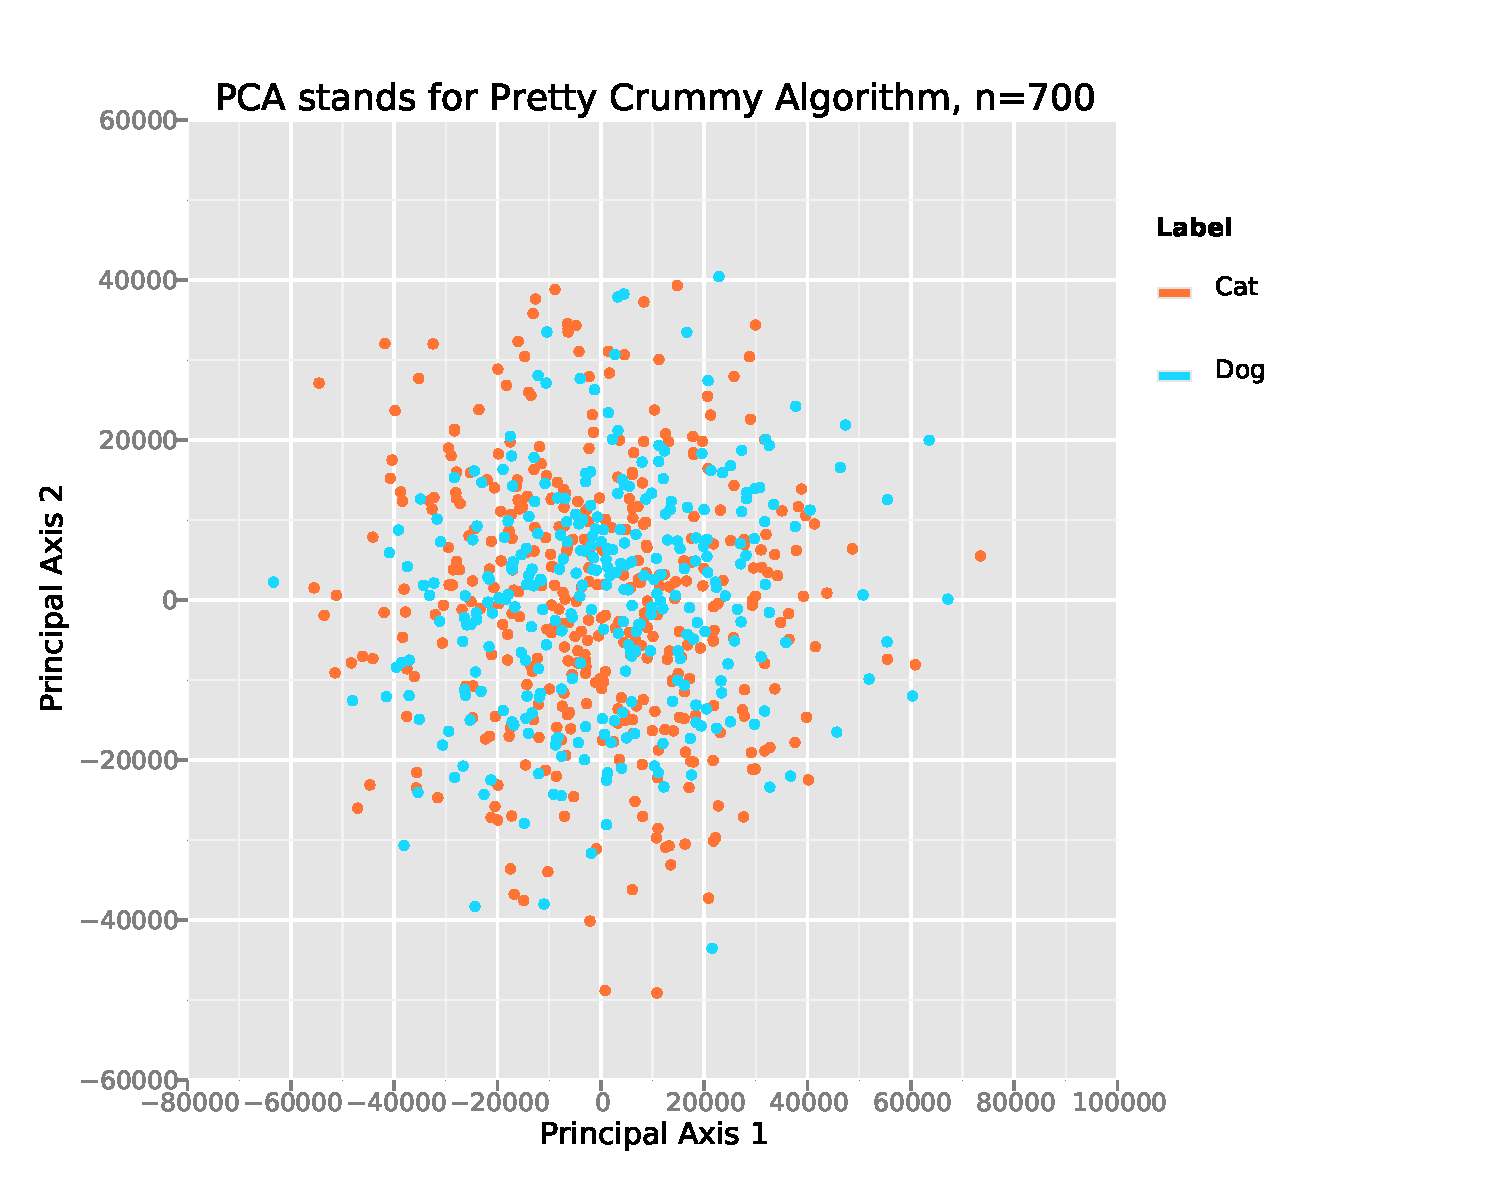
\includegraphics[scale=.50]{PCA_plot.pdf} 
\end{figure}

There is little to no difference between the dog and cat pixel values. This makes sense--we do not distinguish dogs from cats based on just color, and even that is difficult, because this method is not location-independent. A dog in the upper left will produce a completely different loading from a picture with the same dog in the bottom right. With a linear discriminant rule, this approach yields a classification rate less than 55\%. 

Attempting to use support vector machines instead on the principal loadings would allow for a non-linear discrimination rule. This solves very few of our problems, as is clear in its 57\% classification rate.

\subsection{Overfeat Feature Label Classifier}
It is clear that a pixel-only approach is not the best idea. There are too many features that operate on a scale bigger than the pixel level. From a biological perspective, we tend to evaluate dogs and cats on the shape of the ears, bushiness of tails, and the eyes. It would be smart if we had a method for picking out important features that were most indicative of ``cat-ness'' or ``dog-ness''. 

Convolutional Neural Networks (CNN) are trained to extract and identify ``features'' from raw images, with built-in invariance with respect to translations, scaling, or local distortion of the input image. This means that it can pick up a cat in the upper-left and know it's the animal as a picture with the same cat in the bottom-right. This kind of robustness to geometric transformations is achieved by a well-organized coordination between the \emph{convolutional layers} and the \emph{sub-sampling layers} of the network, which are two elements lying in the heart of the CNN design. Those layers, arranged alternately in the network, provide a progressive increase of the richness of the image representation (by convolution), compensated by a progressive reduction of spatial resolution (by sub-sampling). The capability of the CNN to capture local features partially results from the adoption \emph{local receptive fields}, which enforces each unit in a convolutional layer to connect only with a small local neighborhood of units in the previous layer, in contrast to the fully connected layers used in a classical Multilayer Perceptron Network (MLP). The idea behind this design perfectly exemplifies the line of thinking that one usually follows when developing ML algorithms for real-world learning tasks: identify the limitations of the previous algorithms in light of the characteristics of the current problem, and search for improvement. Images tend to have a strong 2D local structure containing highly correlated pixels, but existing algorithms totally ignore the correlation structure of the input. Thus, one has to restrict the connection of each neuron locally in order to extract and combine local features.

The OverFeat program implements a convolutional neural network, which attempts to find important features in an image. The neural network's feature selection is trained on the ImageNet database, a collection of 14.2 million images, each one tagged with relevant classes. This is generally a very time-intensive procedure, but OverFeat pre-trains the convolutional neural net, and classifying on an image takes less than ten seconds, since the CNN is written is C++ and compiled against an optimized BLAS.

The Overfeat program will, by default, output ImageNet categories. This classifier takes the ImageNet corpus for dog and cat words, and deterministically classifies an image as Dog or Cat, based on whether the most common feature word is a dog or cat word. If an image contains neither dog nor cat words, the image is randomly placed in Dog or Cat with equal probability. This method is very naive, and doesn't use any further machine learning techniques to classify, but still manages to drastically outperform pixel-based methods. On the training set, this method manages to correctly predict 88.7\% of the images. This demonstrates, more than anything, the power of the convolutional neural network in classifying images, as the classifier itself is extremely primitive.

\subsection{Overfeat Layer Classifiers}
In this approach, we extract the neural net layers from the Overfeat feature selection algorithm, pre-trained on ImageNet. This produces a large three-dimensional matrix of features. We apply the method of max-pooling, where we take the node with the largest activation, which involves taking the maximum over all columns, then the maximum over the depth of the matrix. The purpose is to reduce the feature space into something more manageable to avoid overfitting. This produces a 4096 x 1 vector from each image. The hard work complete, we try two classifiers to get the final labels.
\begin{description}
\item[SVM:] We use the labels and 4096-vectors to build a support vector machine with a variety of kernels on a subset of the data. Linear, cubic, and radial basis were used as kernels. Cross-validation on the training data gives us an estimate of which kernels will perform the best on the testing set. The extra complexity of the RBF proves useful, and it scores a slightly better classification rate. Cross-validated, our classification rate is 97.5\%, with linear and cubic kernels coming up a few percent behind.

\item[Neural Net:] We build a back-propagated neural network with 4096-length input layer and a 1D output layer. We play around with the number of hidden neurons and train until suitable number of iterations passes and our in-sample and out-of-sample error rates seem to converge. We use the trained neural net to predict testing observations for a classification rate of 96.9\%.
\end{description}

\section{Results}
Using the CNN-SVM approach (since it scored the highest classification rate), we run the trained OverFeat program on the computing cluster to generate feature vectors in parallel. This task still took almost a day, due to the large number of images and availability of resources on the cluster, but finished far faster than if it were run sequentially on a laptop. These 20,000 images were fed into the Support Vector Machine, with labels, as training data. The 5,000 test images were then run in parallel on the cluster to get their feature vectors as well, and their feature vectors were classified against the existing model built up through the training data. A few images did not manage to produce sensible results from OverFeat, or simply failed. This occurred in about 100 images, and they were then handled serially, enlarging the images to make them produce output. The images with the 50 worst certainties were removed, since we were allowed to not classify at most 50 images. The hope is that this would slightly bring up our classification rate. The images that did not classify nicely usually didn't if the dog or cat was not shot head on, or the profile of the animal looked different. A couple images did not classify nicely because they were not cats or dogs at all. The program also had trouble with very small images.

\begin{figure}[H] \center
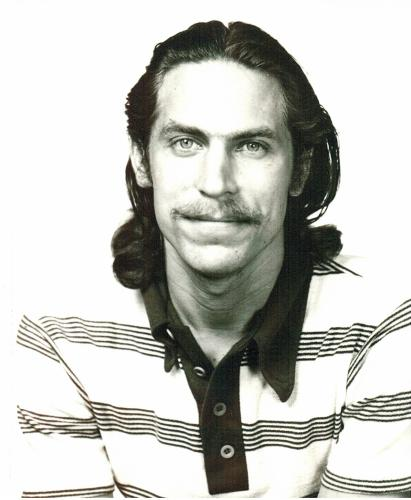
\includegraphics[scale=.25]{hard/3577.jpg} 
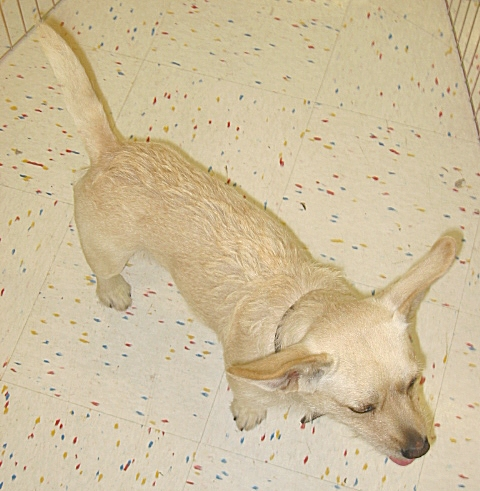
\includegraphics[scale=.25]{hard/3989.jpg} 
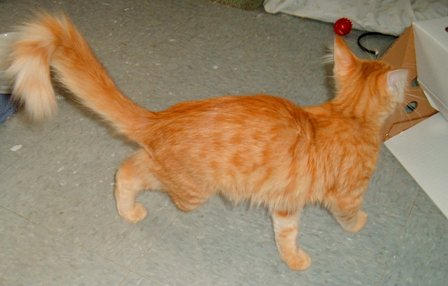
\includegraphics[scale=.50]{hard/4202.jpg} 
\caption{Some images that were difficult to classify (Images 3577, 3989, and 4202)}
\end{figure}

We submitted predictions using linear, cubic, and radial basis functions as our SVM kernels. At best, using the RBF kernel, we managed to get a 97.4\% classification rate on the final data set.

\section{Future Work}
We were about two percent away from achieving the world record classification score on this task, but this still does not put us in the top ten, even! We would be curious to see how we could acquire a higher classification rate. One thought is to use something more sophisticated than a simple SVM as our classifier. It was noted that the linear kernel did several percent worse than a more complicated kernel, so what if we chose to use a deep learning neural network as our classifier, too? It is possible a second deep network could give us even one or two points more accuracy.

The program was quite unstable. OverFeat started from a system call from within Python, but finishing execution on one image in a loop did not kill the completed instance of OverFeat. Thus, after several iterations of the loop through the images, OverFeat would have errors. A quick work-around was to kill any existing OverFeat instances during each iteration of the loop, but this seems rather forced and silly. It would be nice to figure out why instances weren't completing after they outputted their layers. 

Additional work could be done to acquire more images to train our classifier. I imagine we would've gotten closer to the record if instead of 20,000 labeled images we were able to use closer to then 14 million in use on ImageNet. The gains would not be much greater than using 20,000 images from the training data, but it may have made a slight difference.

\section{Most Important Things Learned}
The spherical version of the k-means clustering algorithm was unfamiliar to all of us, as were the damped k-means updates advocated in the paper. Additionally, we learned that it's important to set clear project goals early on; our group was somewhat directionless until halfway through the quarter.
 
All three of us were beginners to machine learning, and picked up the basics of some important ML algorithms and techniques. We experimented with several classical supervised learning methods when trying to select a classifier to apply to our feature layer extracted from OverFeat.  We learned a great deal about convolutional neural networks. For the multilayer perceptron classifier, Chuan read into the architecture behind the algorithm and learned the gradient \emph{back propagation} algorithm, trying to understand how it works and how it can be applied to multi-layer neural networks and solve complicated learning tasks like this one.

Having little experience with machine learning, we also hadn't done much programming with machine learning. We have become more comfortable writing Python code to accomplish machine learning tasks, and why machine learning and Python are a great match. The Scikit-Learn machine learning library in Python makes it incredibly easy to train, tune, predict, and get measures of uncertainty. The library is written largely in C, making everything much faster than if it had been written by hand in Python or R.

Another useful tip we learned was that after selecting the machine learning algorithm, most of the time was spent on rather mundane tasks. For example, reading and cleaning the training data, and analyzing how to present data to the learning algorithm took the better part of three or four weeks. Simply figuring out how to get the predictions from the OverFeat program into a form that the classifier would like took at least two weeks, and even the final output could've used more structure to prevent Segmentation Faults from OverFeat, which happened constantly. This shows that ML skills can only be acquired through an integration of theoretical training and coding practice--theory will only carry one so far before implementation must be worked out.

\section{Appendix}
\subsection*{Explanation of Code}
Our source code can be found on our Github repository: \url{https://github.com/nick-ulle/STA298S14}. Each folder is associated with a particular approach we took towards classifying the testing set. The final approach we took is in the folder ``Overfeat\_Layer\_Classifiers''. The important source code files are described in detail:
\begin{description}
\item[ExtractLayers.py:] The code that extracts layers using the OverFeat neural network. The program determines the directories of all images and output folder, then makes a system call to the OverFeat program on each file. If run on the computing cluster, it takes an argument from the command line that tells it the number of the image it is going to extract. It prepends ``cat'' or ``dog'' on the number to get the corresponding cat and dog images to train. OverFeat is then run on each file. If OverFeat fails to generate a layer matrix because the image is too small, the image is doubled in size and run again. After max-pooling, it writes out the 4096-vector for cat and dog to a CSV file and exits.
\item[Gauss\_batch.sh:] File containing parameters for the Gauss cluster job, to be run on all 20,000 training images.
\item[TrainLayers\_SVM.py:] Trains a support vector machine on the 20,000 images, and tests the classification rate using a really crude cross-validation scheme. Uses linear, cubic, and RBF kernels, and outputs their predictions on a held-out set of the training data.
\item[Test Predictions/ExtractLayers\_Fix.py:] The cluster failed on numerous jobs in the testing set. This fix file was run on my local machine, and implements a loop over the images instead of a cluster job. It is more or less the same file, but designed to be run with much more control and hand-holding.
\end{description}

\subsection{References}
\begin{description}
\item[] Philippe Golle. 2008. Machine learning attacks against the Asirra CAPTCHA. In Proceedings of the 15th ACM conference on Computer and communications security (CCS '08). ACM, New York, NY, USA, 535-542. DOI=10.1145/1455770.1455838 http://doi.acm.org/10.1145/1455770.1455838
\item[] Adam Coates, Andrew Ng. 2012. Learning Feature Representations with K-means. In Neural Networks: Tricks of the Trade, Reloaded, Springer LNCS.
\end{description} 
\end{document} 
